\documentclass[a4paper]{article}
\usepackage{float}
\usepackage{fullpage, amsmath, amssymb, verbatim} % Package to use full page
\usepackage{graphicx}
\usepackage{adjustbox}
\usepackage{url}

\title{Deep Learning: Assignment Three}
\author{Aditi Nair (asn264) and Akash Shah (ass502)}
\date{May 2, 2017}
\begin{document}

\maketitle

\section{Generative Adversarial Networks}

\begin{enumerate}
\item{\textit{Explain generative modeling.} 
\newline
\newline
A generative model uses training data drawn from an unknown distribution $p$, and learns a representation of the distribution, called $\hat{p}$. Generative models can represent $\hat{p}$ directly, generate samples from $\hat{p}$, or both. 

}
\item{\textit{Compare Generative Adversarial Networks (GANs) with other Unsupervised learning approaches, such as Auto-encoders. Explain the difference.}
\newline
\newline
We can compare GANs with other models that estimate probability distributions by choosing distributions that maximize the likelihood of the observed training data. Within this category, we can distinguish between generative models that implicitly and explicitly represent the probability density function $\hat{p}$. 
\newline
\newline
For explicit density models, the maximum likelihood estimation (MLE) task involves choosing probability density functions for $\hat{p}$, and then using gradient descent methods to appropriately parametrize the density functions. Creating MLE-driven generative models that develop explicit density functions are challenging because effectively estimating probability distributions often requires complex models, whose optimization can be computationally intractable. Currently, this is addressed by carefully constructing tractable explicit density functions (like Fully Visible Belief Nets, or FVBNs) and by constructing intractable explicit density functions (like Variational Auto-encoders, or VAEs), which require approximations to complete the MLE task. We will focus on comparing FVBNs, VAEs and GANs since they are currently three of the most popular approaches to generative modeling.
\newline
\newline
FVBNs use the rule of conditional probabilities to represent a distribution $\hat{p} \left( \textbf{x} \right) $ over an $n$-dimensional vector $\textbf{x}$:
$$\hat{p} \left( \textbf{x} \right) = \prod_{i=1}^n \hat{p} \left( x_i | x_1,...x_{i-1} \right) $$
That is, the probability distribution over $\textbf{x}$ is defined as the product of the conditional probabilities over its individual components. In particular, this operation cannot be parallelized because of the conditional nature of the computation. In WaveNet, a popular approach to FVBNs, each $\hat{p} \left( x_i | x_1,...x_{i-1} \right)$ is computed by a neural network. Accordingly, the computation of each conditional probability can be expensive, and can only be executed sequentially, making it difficult to scale the model for more demanding tasks. 
\newline
\newline
Next, we consider VAEs, which fall in the category of explicit density models which rely on approximation to complete the MLE task. Intuitively, VAEs use encoders to transform high-dimensional input vectors $x$ into a lower-dimensional latent space representations $z$, and then attempt to re-construct the original vectors using decoder networks. Probabilistically, we can argue that we would like to calculate the posterior distribution $p \left(z|x \right) $ so that we have good estimates for $z$ given the training data $x$. In variational inference, we approximate this distribution with $\hat{p} \left( z|x \right)$. In order to optimize our choice of $ \hat{p} \left(z|x \right)$ we would like to minimize the Kullback-Leibler divergence:
$$KL\left( \hat{p} \left(z|x \right) |  p \left( z|x \right) \right)  = \int_{x} \hat{p}(z|x) log \frac{\hat{p}(x|z) }{p(z|x ) } $$
$$ = \int_{x} \hat{p}(z| x) log \ \hat{p}(z |x)  - \hat{p}(z| x) log \ p(z|x )  $$
$$ = \mathrm{E}_{\hat{p}} [ log \  \hat{p}(z |x) ] - \mathrm{E}_{\hat{p}} [ log \ p (z | x) ]  $$
By Bayes' Rule:
$$ p (z|x) = \frac{p(x,z)}{p(x)}$$
So we can write:
$$KL\left( \hat{p} \left(z|x \right) |  p \left( z|x \right) \right) = \mathrm{E}_{\hat{p}} [ log \  \hat{p}(z |x) ] - \mathrm{E}_{\hat{p}} \Big[ log \ \frac{p(x,z)}{p(x)} \Big] $$
$$ =   \mathrm{E}_{\hat{p}} [ log\  \hat{p}(z |x) ] - \mathrm{E}_{\hat{p}} [ log \ p(x,z) ] + log \ p(x)$$
Clearly the term $log \ p(x)$ is intractable. Either we must know the distribution $p(x)$ - in which case we have already solved the problem of generative modeling - or we must compute it by marginalizing over $z$ - $\int_z p(x|z) p(z) dz$ - which is intractable since the space of all possible $z$ is large. However, we observe that by maximizing the following tractable expression:
$$\mathrm{E}_{\hat{p}} [ log \ p(x,z) ] - \mathrm{E}_{\hat{p}} [ log\  \hat{p}(z |x) ] $$
we minimize the KL-divergence as written above. Therefore, in the VAE setting, we choose to maximize the above expression, known as ELBO, instead. However, optimizing over the ELBO only provides a lower bound over the original KL-divergence, which has an added $log \ p(x)$ term. In addition, if we choose an inappropriate distribution for the prior or the posterior of $\hat{p}$, then we end up selecting $\hat{p}$ poorly. This is the primary weakness of VAE models, in addition to the lower quality of their generated samples.
\newline
\newline
Finally, we consider GANs. A GAN can be described as a game between two adversarial players, a generator $G$ with parameters $\theta^G$ and a discriminator $D$ with parameters $\theta^D$. The generator creates samples which appear to be drawn from original distribution $p$. The discriminator classifies samples as being real (drawn from the original distribution) or fake (created by the generator), and is trained to minimize the following loss:
$$ J^D(\theta^D, \theta^G) = -\frac{1}{2} \mathrm{E}_{x \sim p_{data}} [log\ D(x)] - \frac{1}{2} \mathrm{E}_z [log\ (1 - D(G(z)))]$$
The first summand expresses the cross-entropy loss of the discriminator on real samples drawn from the training data. $D(x)$ expresses the discriminator's probability estimate that $x$ is sampled from the data. If $D(x) = 1$, then $log\ D(x) = 0$ and the left summand is minimized. The second summand expresses the cross-entropy loss of the discriminator on ``fake" samples created by the generator. $z$ are noise vectors sampled from a prior distribution (e.g. a uniform distribution on a unit hyper-cube), which are fed to $G$ to create fake samples. $D(G(z))$ expresses the probability that $z$ is sampled from the data distribution, so $1- D(G(z))$ expresses the probability that $z$ is fake. If $D(G(z)) = 0$, then the discriminator is certain that a fake is indeed fake, and the right summand is minimized. Note that $ J^D(\theta^D, \theta^G)$ is a function of $\theta^D$ and $\theta^G$, but $D$ can only optimize over $\theta^D$.
\newline
\newline
Next, the generator is trained to ``fool" the discriminator. The loss function used for the generator can vary, but a common one is the cross-entropy loss:
$$J^G(\theta^G, \theta^D) = -\frac{1}{2} \mathrm{E}_z [log \ D(G(z))] $$
$J^G$ is a function of $\theta^D$ and $\theta^G$ but $G$ can only optimize over $\theta^G$. If $G(z)$ looks exactly like a sample drawn from $p_{data}$, then $D(G(z)) = 1$ and we will minimize $J^G$.
\newline
\newline
Typically, both the generator and the discriminator are neural networks which are trained simultaneously using gradient descent on real and fake samples. Unlike FVBNs and VAEs, GANs only provide us with an implicit representation of $\hat{p}$, since the generator is a neural network constructed to create the $G(z)$ samples. For the same reason, unlike FVBNs, GANs can generate an entire sample simultaneously. Whereas VAEs require you to carefully select the distribution for the approximator $\hat{p}$, the neural networks used in GANs are generally considered universal approximators. In addition, unlike (most) VAEs, a GAN trained with sufficient data can theoretically recover the true distribution $p_{data}$ - it is clear above that both $J^G$ and $J^D$ can be minimized directly, whereas we can only minimize the ELBO of the VAE loss function. Finally, it is worth noting that GANs are (subjectively) considered to produce better samples than VAEs and FVBNs.
}
\item{\textit{Explain conditional generation using GANs, versus the vanilla unconditional version. Please briefly draw a diagram when training conditional GANs, with the condition context C, generator G, discriminator D, random vector z and output x.}
\newline
\newline
In the previous presentation of GANs, we described ``vanilla" unconditional generation where we take $z$ samples from a noisy prior distribution and feed them into the generator $G$. One problem is that we have no control over the kind of sample we generate - or, mathematically speaking, on the distribution of the samples being generated. 
\newline
\newline
To address this issue, Mirza and Osindero (2014) suggest building Conditional GANs, which condition both the generator and discriminator on some context $C$. For example, Mirza and Osindero set $C$ as one-hot vectors indicating class labels for data. [3]
\newline
\newline
In the generator, we combine the noise vector $z$ with the context $C$ at the input layer (for example, by concatenation), before feeding it through an appropriately-sized convolutional network to generate $G(z|C)$. Ideally, $G(z|C)$ should look like it belongs to the class of $C$. In the discriminator, we similarly combine the inputs $X$ (either $G(z|C)$ or $x \sim p_{data}$) with the appropriate one-hot vector $C$ before feeding it through an appropriately-sized convolutional network to compute $D(X|C)$. Finally, to generate samples of a specific class, we simply sample $z$ from the noise prior, concatenate with the $C$ vector for the intended class and compute $G(z|C)$. 
\newline
\newline
Below, we provide a diagram of the Conditional GAN framework (borrowed from Mirza and Osindero and modified with our notation):
\begin{figure}[H]
  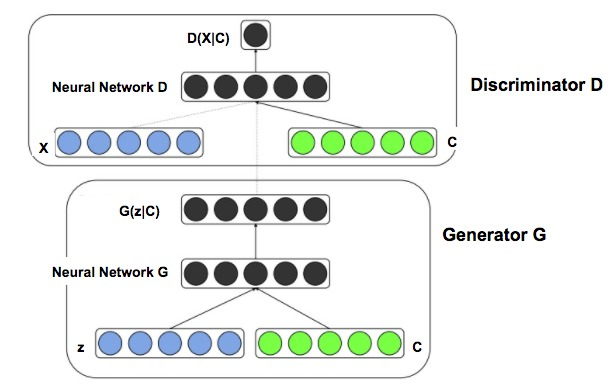
\includegraphics[scale=3]{images/my_conditional_gan.jpg}
  \label{fig:boat1}
\end{figure}

}
\end{enumerate}

\section{GAN Workhouse}

We trained several GANs on the CIFAR-10 dataset. The CIFAR-10 dataset consists of 50,000 training images from 10 classes: airplane, automobile, bird, cat, deer, dog, frog, horse, ship, truck. The images are only 32x32 pixels, and we found that the resolution quality of the images is poor. To begin our exploration of GANs, we decided to train a DCGAN model, developed by Radford et. al., which has generally strong performance on generative tasks for images. [5] We trained our baseline model using the PyTorch implementation (and default parameters) of DCGAN, which can be found in the PyTorch GitHub repository. [6] Below, we show an example of generated output of this baseline model after 40 epochs.
\\
\\
\begin{figure}[H]
  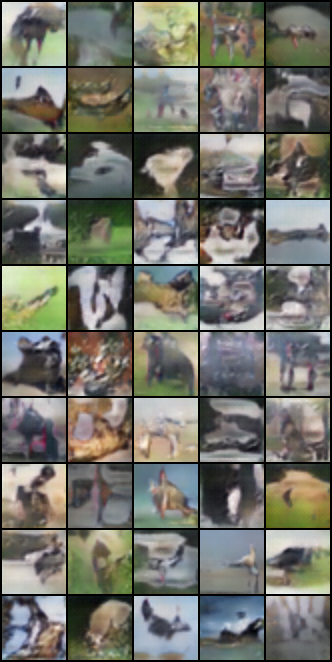
\includegraphics[scale=0.5]{images/baseline_normalized_10x5_generated.png}
  \label{fig:boat1}
  \caption{Baseline Model at 40 Epochs}
\end{figure}

Next we incorporated the conditional GAN framework outlined in Conditional Generative Adversarial Nets into the DCGAN model, so that we could utilize class labels while training on the CIFAR-10 dataset. This would also allow us to do class-conditioned generation of images. As described in the paper, a vanilla GAN can be extended to a conditional GAN by feeding additional information, like class labels or data from other modalities, into both the generator and the discriminator. 
\newline
\subsection*{Conditional DCGAN Architecture}
In the first version of our conditional DCGAN model, we concatenated the input noise vector $z$ and a one-hot encoding of a randomly-chosen class label, then passed this entire concatenated vector into the generator $G$. Besides the class-conditioned input vector $z$, the architecture of the generator was exactly as in the original DCGAN model. 
\newline
\newline
In the discriminator, an image tensor that came from either a real example in the data or from the generator was passed through a series of convolution, leaky ReLU, and batch-norm layers - that is, through a convolutional neural network - to create a single feature vector. Then this feature vector was concatenated with a one-hot encoding of the image's class label. If the image being passed through the discriminator was from the original dataset, then its true class label would be used. If the image was a  fake image created by the generator, then the random class label used for generation was used. Finally, the concatenation of the feature vector and its corresponding one-hot label vector was passed through a sigmoid layer, which used an affine transformation to map the input vector to a single value and then applied the sigmoid non-linearity to compute the required probability. 
\newline
\newline
In this model, we have two new parameters to tune - the dimension of the convolution feature vector in the discriminator that is concatenated with the one-hot label vectors, and the vector representations used to represent class conditionals. First, we experimented with the former by varying the dimensions of the convolved feature vector between 100, 200, and 400. We found that the dimension of 100 resulted in the lowest quality images, while 200 and 400 were fairly similar, though 400 was slightly better. We concluded that more expressive features from the convolutional network resulted in better performance in the overall model. Below we show output from our conditional model with a convolution feature vector dimension of 400, trained for 87 epochs:
\begin{figure}[H]
  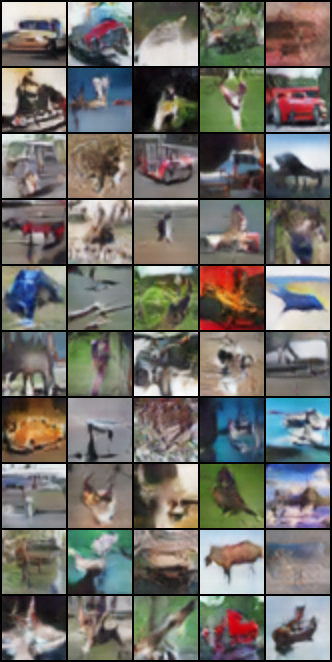
\includegraphics[scale=0.5]{images/conditional_400_10x5_generated.png}
  \label{fig:boat1}
  \caption{Generated Images from Our Best Model}
\end{figure}
In the grid above, each row of images is conditioned on the same class conditional in the following order. By row, the order the class conditionals is: airplane, automobile, bird, cat, deer, dog, frog, horse, ship, truck. Compared to the baseline model, this model generates clearer images with a larger range of colors and tones. Local subsections of these fake images seem like realistic subsections of actual images, though the images lack a overall coherence. However, the improvement in image quality may be partially due to the longer training time of this model.
\newline
\newline
When using the conditional DCGAN model to generate class-conditioned images, we conducted an experiment to determine the extent to which the class conditionals affected the images created by the generator network. We fed the generator the same fixed noise vector with each of the class labels to see if the model generated appropriate images for each class. However, we noticed that all of the images generated from the same noise vector were very similar, even though they were conditioned on different class labels. Below, the ten images in each row are generated from the same noise vector, but conditioned on a different one of the ten class conditionals:
\begin{figure}[H]
  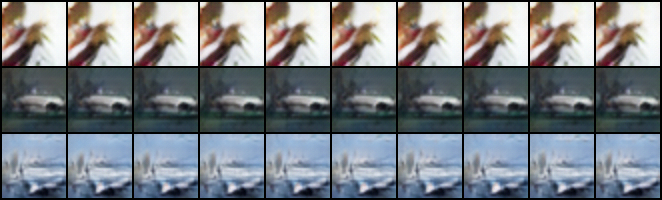
\includegraphics[scale=0.5]{images/conditional_400_fixed_noise_conditional_fake.png}
  \label{fig:boat1}
  \caption{Conditional Experiment on Our Best Model}
\end{figure}
Since CIFAR-10 is a fairly complex dataset, we also trained the same architecture on the popular MNIST dataset, which is generally considered to be ``easier" for the generation task. Below, we show the results of the same experiment after ten epochs - a single fixed noise vector being passed through the generator, each time conditioned on a different class label (in this case, digits):
\begin{figure}[H]
  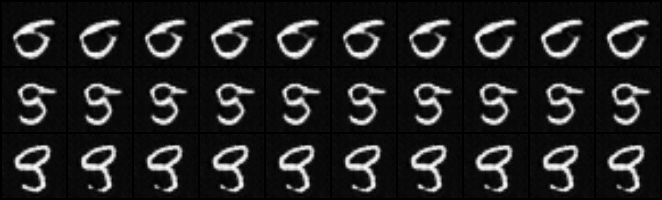
\includegraphics[scale=0.5]{images/MNIST_fixed_noise_conditional_fake.png}
  \label{fig:boat1}
  \caption{Conditional Experiment on MNIST Model}
\end{figure}
In both examples, you can see that the class conditional makes very little difference in the nature of the image generated by the model. However, it is also worth noting that the MNIST model was only trained for 10 epochs (though on an easier dataset), and the CIFAR model was trained for 87 epochs. It is possible that these models need to train much longer to effectively account for the class conditionals.
\subsection*{Experiments with Conditional DCGAN Architecture}
The limited effect of the class conditionals motivated us to modify our architecture so that the model be more sensitive to the class labels in the discriminator and the generator. We thought one issue might be that the magnitude of the values in the feature vector produced by the convolution network of the discriminator might be much larger than the values of the one-hot encoding vector, which contains nine 0 values and one 1 value. We addressed this by adding a batch-normalization layer to the convolved feature vector of the image before it is concatenated with the one-hot class conditional vector. However, this did not work well at all and the images produced resembled pure noise.
\newline
\newline
Next, we considered the possibility that rather than using one-hot vectors, it might improve the model to learn a non-linear embedding over the one-hot class conditional vectors. In one set of experiments, we added a sigmoid layer to the one-hot vector before concatenating it with the convolved feature vector over the (fake or real) image in the discriminator. This sigmoid layer allowed us to learn small (10-dimensional) embeddings over the class conditionals. We also explored adding additional linear and non-linear layers to the discriminator after the concatenation operation. However, after 30-40 epochs of training, these models were not significantly better than the one presented above (at 40 epochs).
\newline
\newline
In another set of experiments, we learned a much larger (200-dimensional) embedding over the one-hot class conditionals before concatenating them with the convolved feature vectors of the (fake or real) image in the discriminator network. This concatenated vector was passed through a sigmoid layer to get a probability value. Below, you can see images generated by this network after 40 epochs of training:
\begin{figure}[H]
  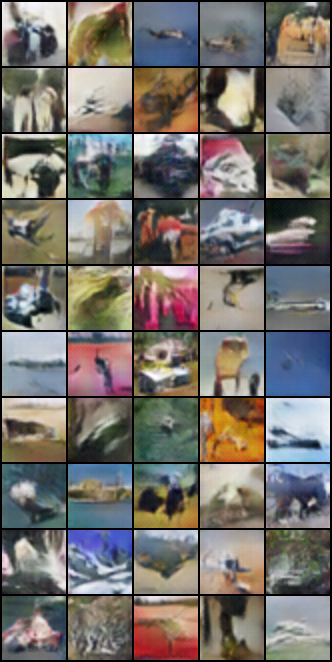
\includegraphics[scale=0.5]{images/LARGE_EMBEDDING_10x5_generated.png}
  \label{fig:boat1}
  \caption{Generated Images from New Conditional Architecture}
\end{figure}
These images approximately match the quality of images generated by our best model (above) after 40 epochs of training. While these images are about as good as the images from our earlier architecture, they were also not especially successful on the conditional experiment described above.
\begin{figure}[H]
  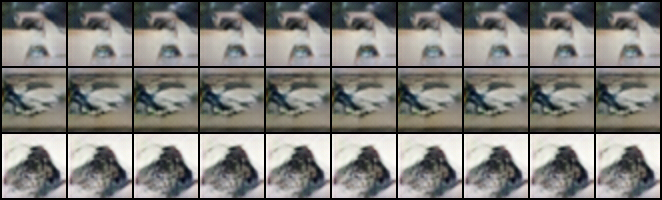
\includegraphics[scale=0.5]{images/LARGE_EMBEDDING_fixed_noise_conditional_fake.png}
  \label{fig:boat1}
  \caption{Conditional Experiment on New Conditional Architecture}
\end{figure}
However, this model has only been trained for 40 epochs. Since it is at least as good as our best model (above) was at 40 epochs, and since this architecture is configured to more easily recognize variations in the class conditionals, we believe that in future experiments this architecture would be more successful in generating high-quality images and in generating different image modalities base don the class conditionals.
\newline
\newline
Finally, in other experiments, we also allowed the generator to learn a 200-dimensional embedding over the one-hot class conditionals, and concatenated these embeddings with noise vectors before passing the concatenated vectors through the generator to create fake images. Unfortunately, this model trained poorly and did not generate images which were comparable to the previous models. 
\subsection*{Conclusion}
In ``Conditional Generative Adversarial Nets for Convolutional Face Generation", Gauthier trained similar models on images of human faces. [4] In these models, it took approximately 130 epochs of training to obtain high quality generated face images, while between epochs 60 and 80, the generated images had some local qualities of faces such as color patterns and borders but not strong global resemblance to faces. Due to computational resources, we were able to train many of our models in the range of 40 to 60 epochs, and, as in the paper, we noticed that our generated images had some local qualities that resembled images from the original data.
\newline
\newline
However, we suspect more training time is needed to get high-quality generated images. We did not train our models with GPUs, but we expect that utilizing GPUs would have allowed some of our models to quickly train past 100 epochs, where we could expect higher quality generated images. Furthermore, the low resolution quality of the original images negatively impacted the quality of our generated images. In future experiments, we would like to train our final architecture (corresponding to the last pair of images above) for over 100 epochs to see how this improve the quality of generated images.
\section*{References and Resources}
\begin{enumerate}
\item{NIPS 2016 Tutorial: Generative Adversarial Networks, Ian Goodfellow. 2016. }
\item{``Tutorial - What is a variational autoencoder?". Jaan Altosaar. Blogpost at: https://jaan.io/what-is-variational-autoencoder-vae-tutorial/}
\item{Conditional Generative Adversarial Networks. Mehdi Mirza and Simon Osindero. 2014. }
\item{``Conditional Generative Adversarial Nets for Convolutional Face Generation" Jon Gauthier. 2015. }
\item{``Unsupervised Representation Learning with Deep Convolutional Generative Adversarial Networks". Alec Radford, Luke Metz, and Soumith Chintala. 2015. }
\item{PyTorch DCGAN implementation by FAIR: https://github.com/pytorch/examples/tree/master/dcgan}
\end{enumerate}
\end{document}
